\section{Studies of signal and background separation in detector-level of cluster}
In the future detector, when the luminosity is increased, the pileup is bigger, and it will be more difficult to distinguish the signal and the background. In this section, we want to study different variables and see their ability to separate the signal and the background in different detector sizes in the clustering of detector-level.\\

Figure 3 to 5 show the ROC curves of three variables, $c2b1$ , $\tau_{21}$, and $\tau_{32}$. For each variable, there are three different sizes of the sub-detector HCAL compared at four special collision energies. For different sizes, the one with the highest background rejection rate, which is 1-background efficiency, at the same signal efficiency has the best separate ability.

In Figure 3 for the variable $c2b1$ , all ROC curves of the detector sizes are closed to each other for every cases of energy. So the the detector size is not sensitive to the separate ability in this variable.

For the tau21 variable in Figure 4, at 5 TeV, the smallest detector size (1$\times$1 cm) can separate the background from the signal well. However, this is not the usual case as the ROC curves nearly merge together at higher collision energy. In addition, the detector with the bigger size tends to have higher separation ability than the smaller detector size in 20 and 40 TeV collision energy. 

Figure 5 show variable $\tau_{32}$, the smallest detector size has the best separate at all the cases of energy. This is what we want to see, because we want to use the smaller detector size to enhance the separation ability.

In conclusion,in all the cases of energy and detector size, the variable $c2b1$ has the better separation ability than the other two variables. In addition, the variable $\tau_{32}$ follows the rule that the smaller detector size has the better separation ability. We think this two variables could help to separate the signal and the background in the future detector analysis.\\
\label{sec:efficiency}


\begin{figure}
\begin{center}
   \subfigure[5 TeV] {
   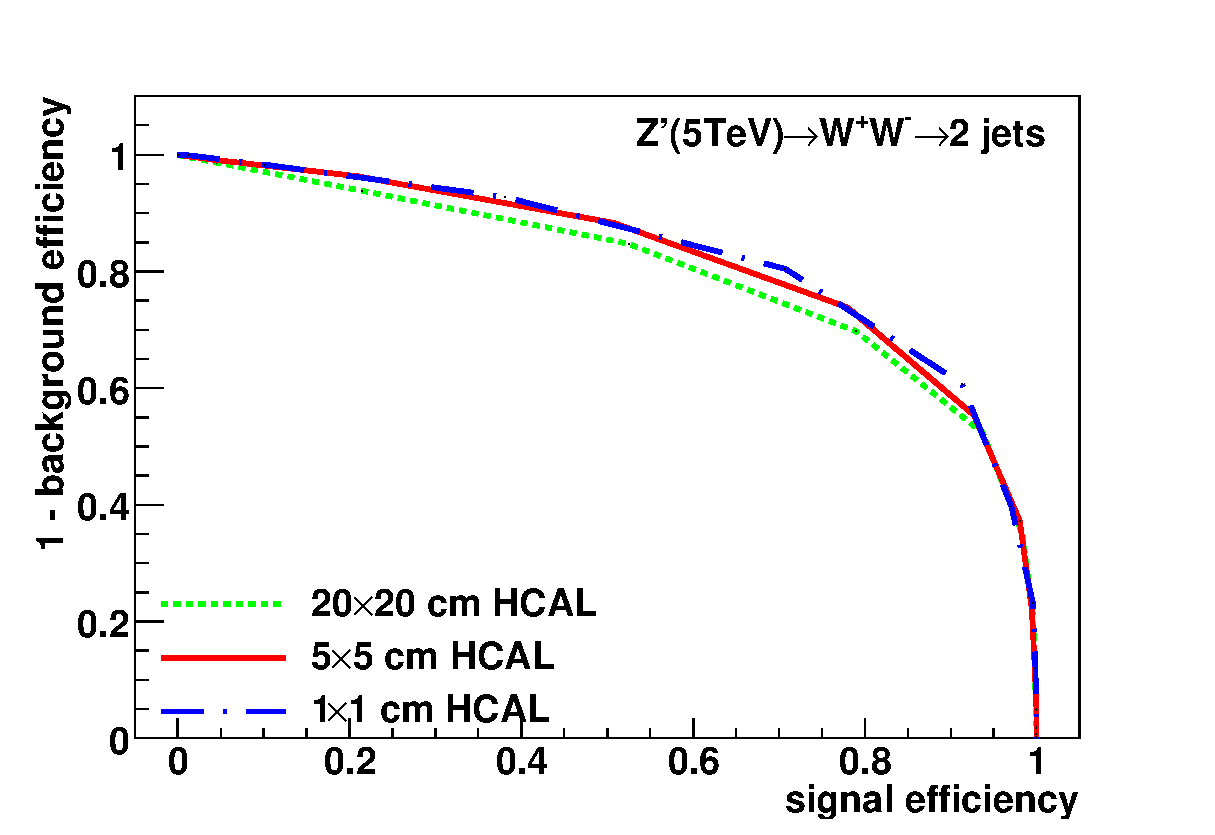
\includegraphics[width=0.43\textwidth]{figs/cluster_c2b1_5_tev_eff.eps}\hfill
   }
   \subfigure[10 TeV] {
   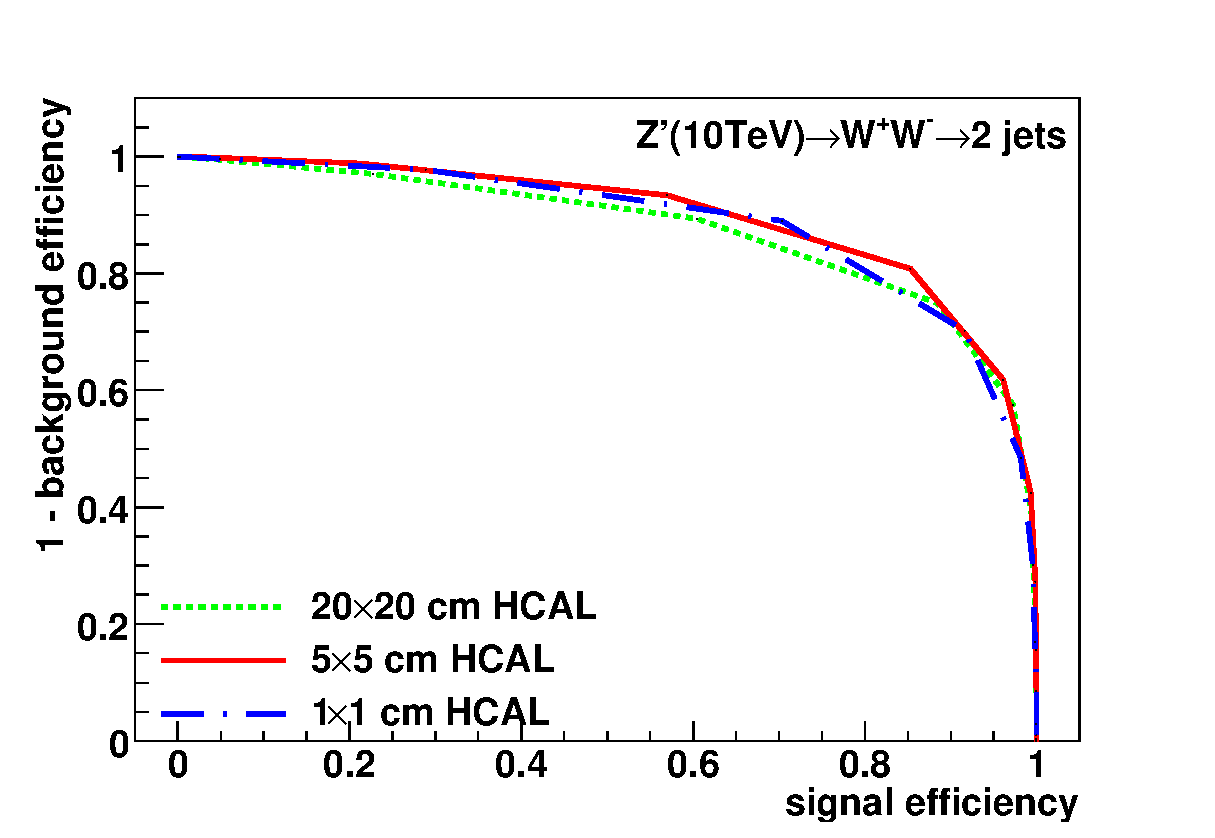
\includegraphics[width=0.43\textwidth]{figs/cluster_c2b1_10_tev_eff.eps}
   }
   \subfigure[20 TeV] {
   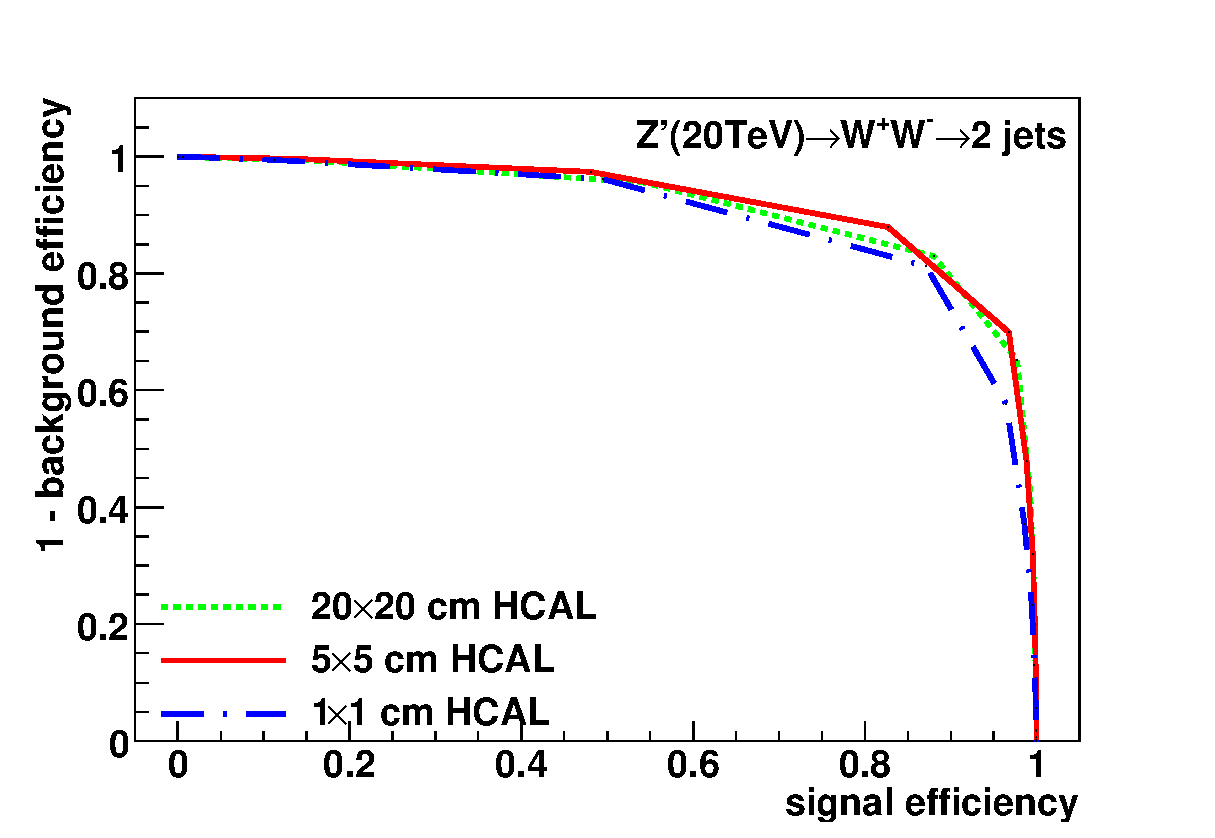
\includegraphics[width=0.43\textwidth]{figs/cluster_c2b1_20_tev_eff.eps}
   }
   \subfigure[40 TeV] {
   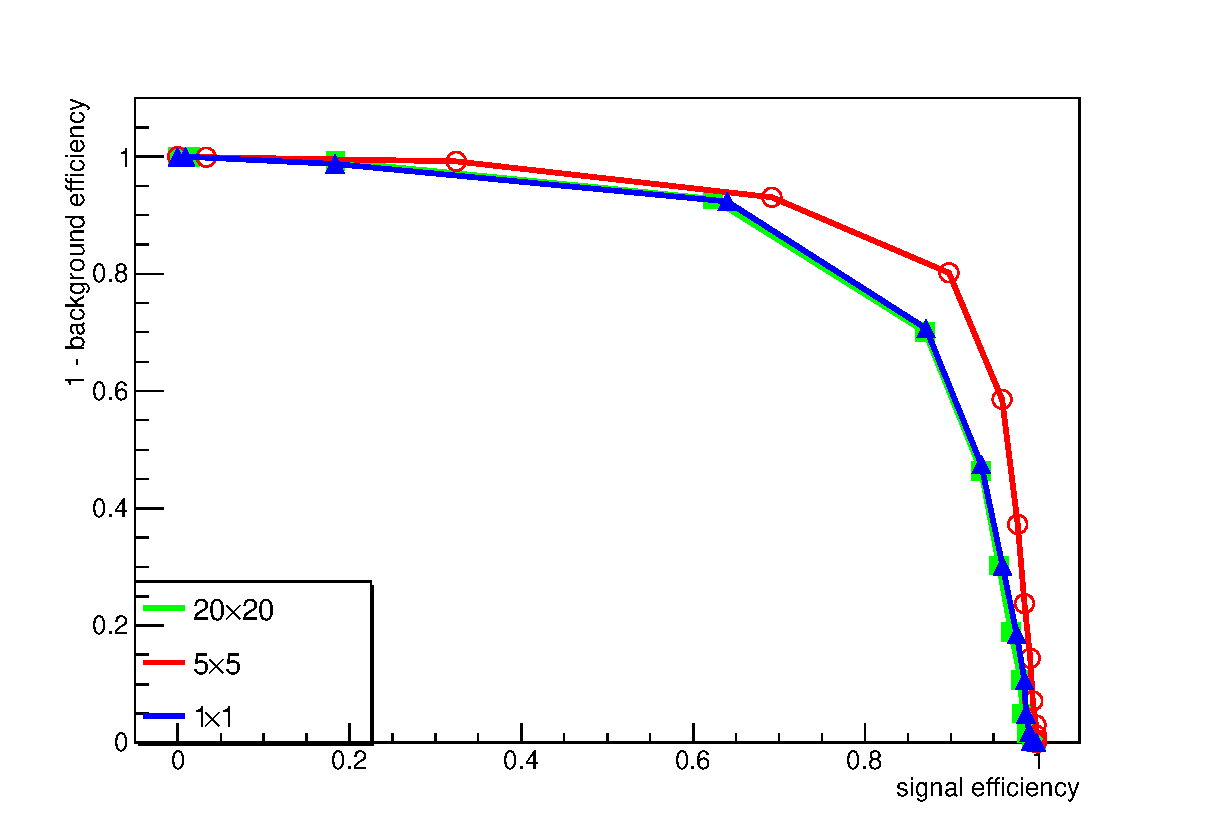
\includegraphics[width=0.43\textwidth]{figs/cluster_c2b1_40_tev_eff.eps}
   }
\end{center}
\caption{Signal efficiency versus background rejection rate using $c2b1$.The energies of collision at (a)5, (b)10, (c)20, (d)40TeV are shown here. In each picture of the energy, there are three ROC curves corresponding to different detector sizes.}
\label{fig:cluster_c2b1}
\end{figure}


\begin{figure}
\begin{center}
   \subfigure[5 TeV] {
   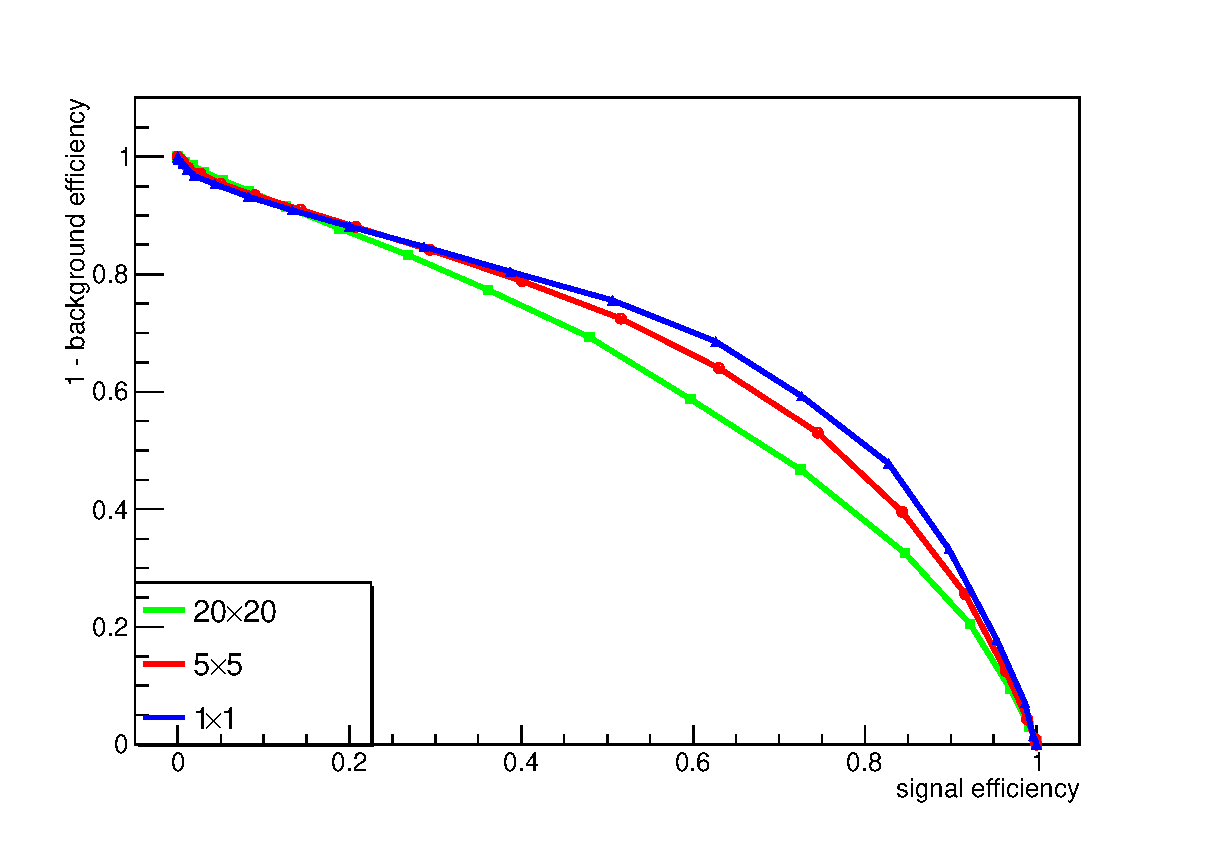
\includegraphics[width=0.43\textwidth]{figs/cluster_tau21_5_tev_eff.eps}\hfill
   }
   \subfigure[10 TeV] {
   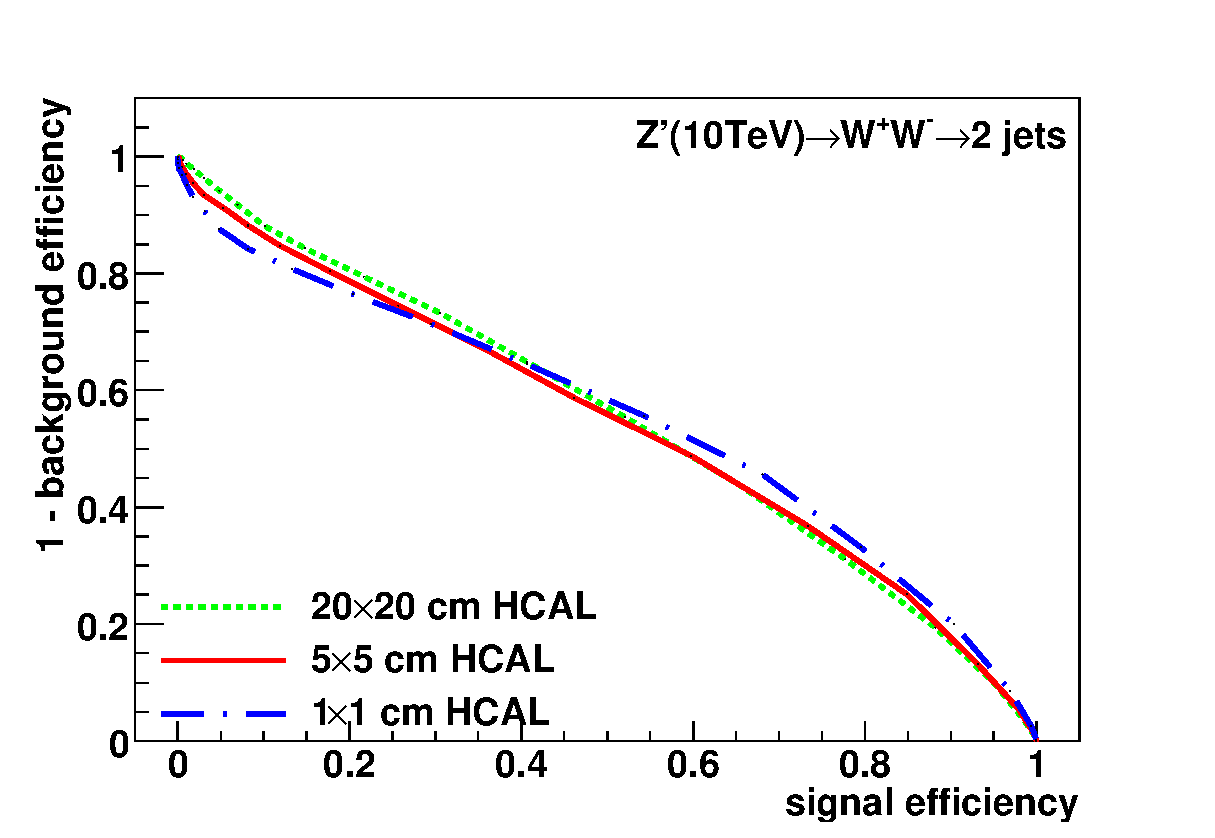
\includegraphics[width=0.43\textwidth]{figs/cluster_tau21_10_tev_eff.eps}
   }
   \subfigure[20 TeV] {
   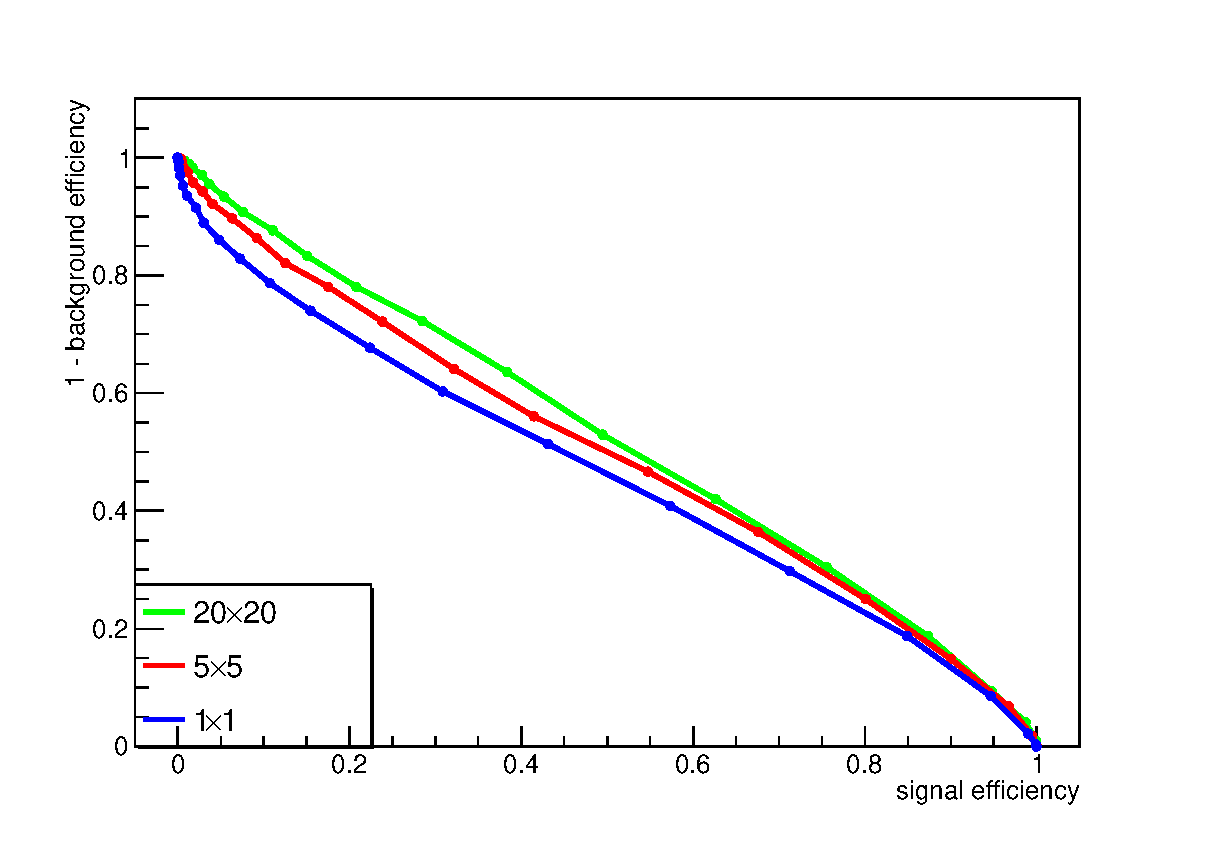
\includegraphics[width=0.43\textwidth]{figs/cluster_tau21_20_tev_eff.eps}
   }
   \subfigure[40 TeV] {
   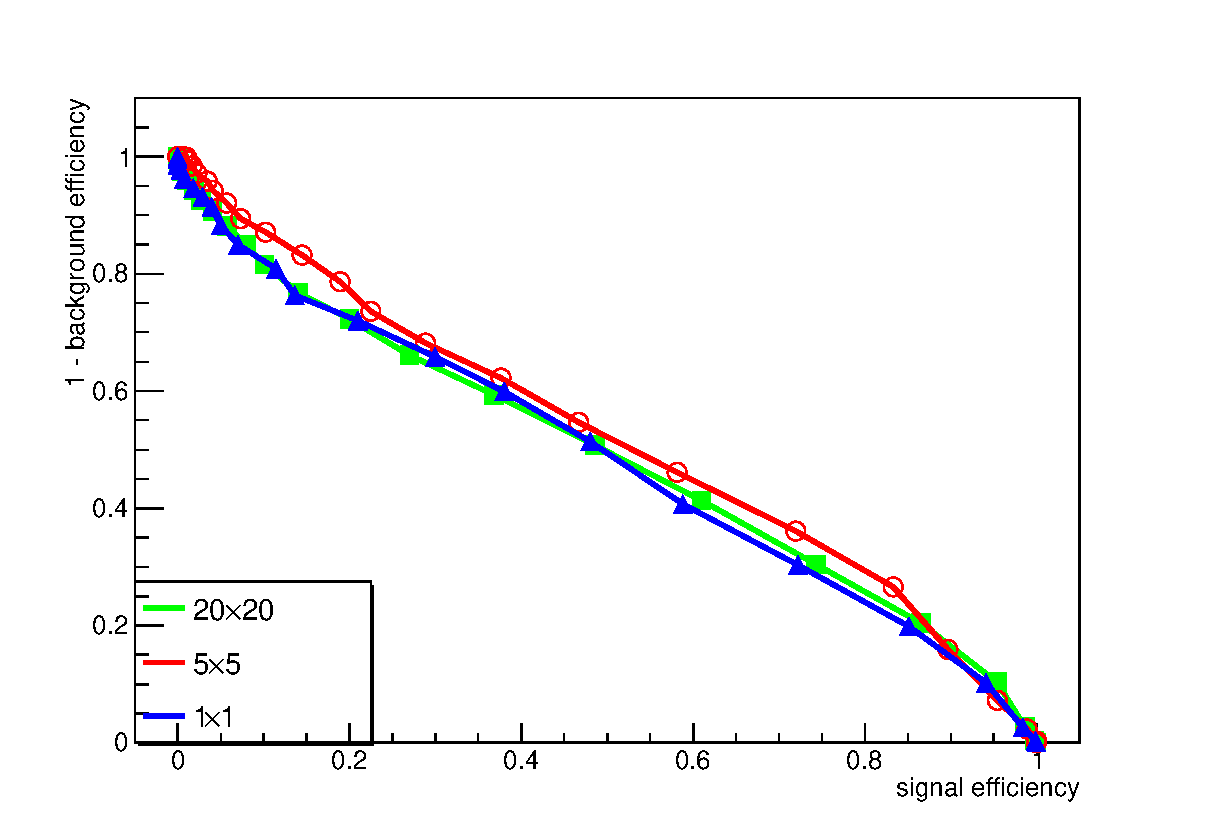
\includegraphics[width=0.43\textwidth]{figs/cluster_tau21_40_tev_eff.eps}
   }
\end{center}
\caption{Signal efficiency versus background rejection rate using $\tau_{21}$.The energies of collision at (a)5, (b)10, (c)20, (d)40TeV are shown here. In each picture of the energy, there are three ROC curves corresponding to different detector sizes.}
\label{fig:cluster_tau21}
\end{figure}


\begin{figure}
\begin{center}
   \subfigure[5 TeV] {
   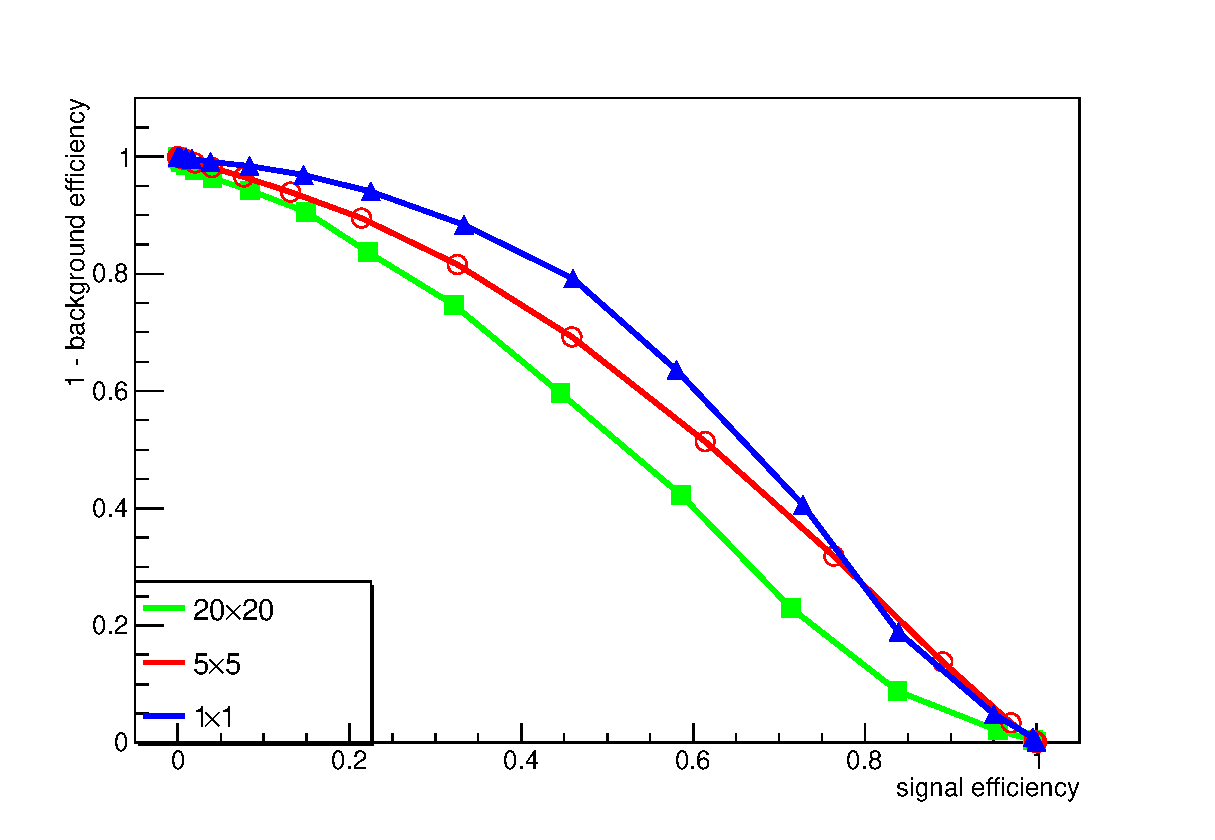
\includegraphics[width=0.43\textwidth]{figs/cluster_tau32_5_tev_eff.eps}\hfill
   }
   \subfigure[10 TeV] {
   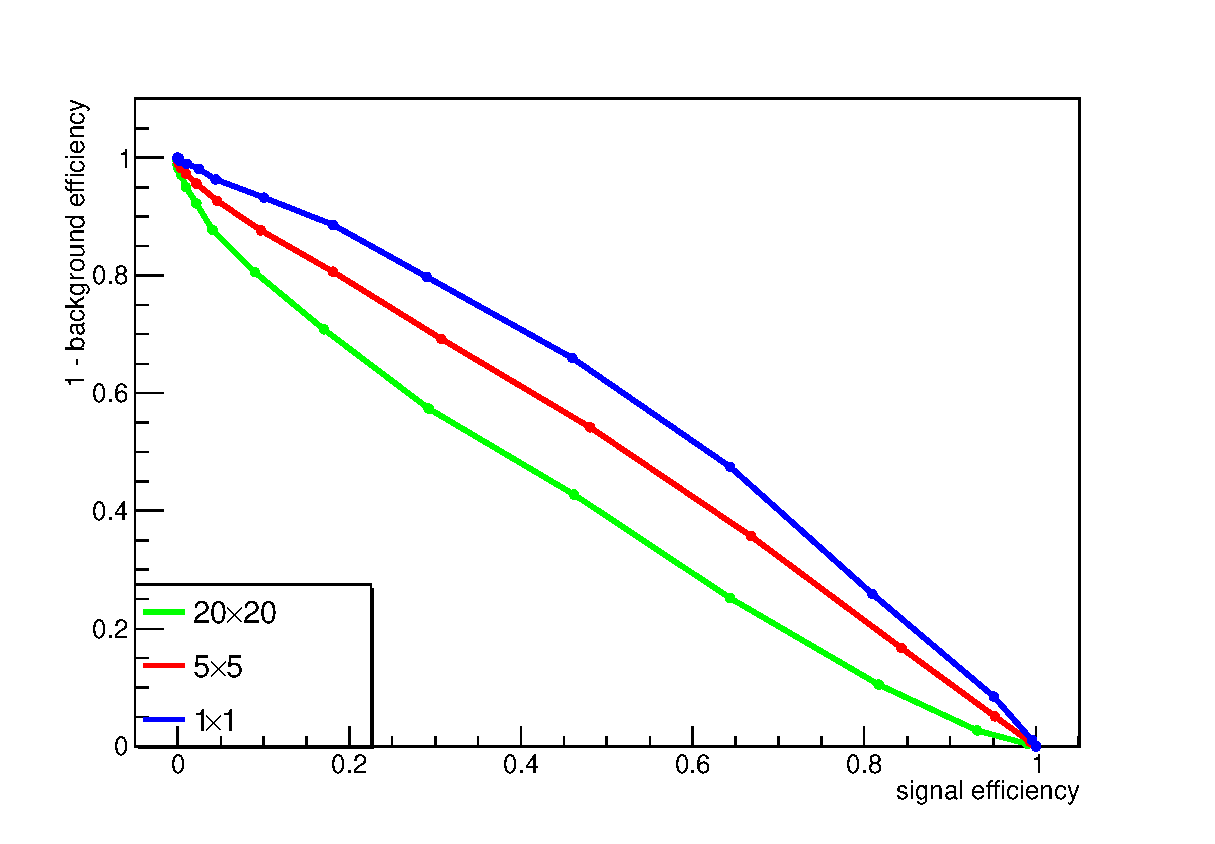
\includegraphics[width=0.43\textwidth]{figs/cluster_tau32_10_tev_eff.eps}
   }
   \subfigure[20 TeV] {
   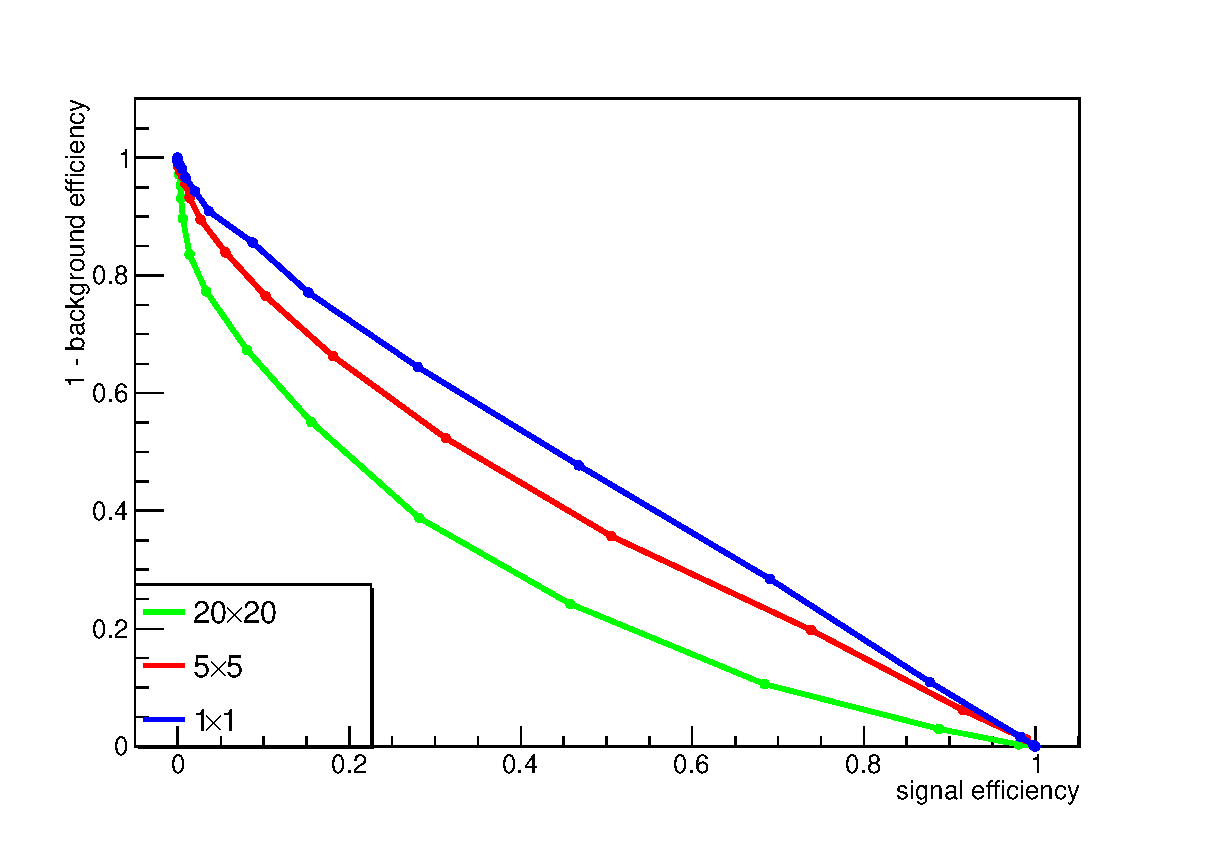
\includegraphics[width=0.43\textwidth]{figs/cluster_tau32_20_tev_eff.eps}
   }
   \subfigure[40 TeV] {
   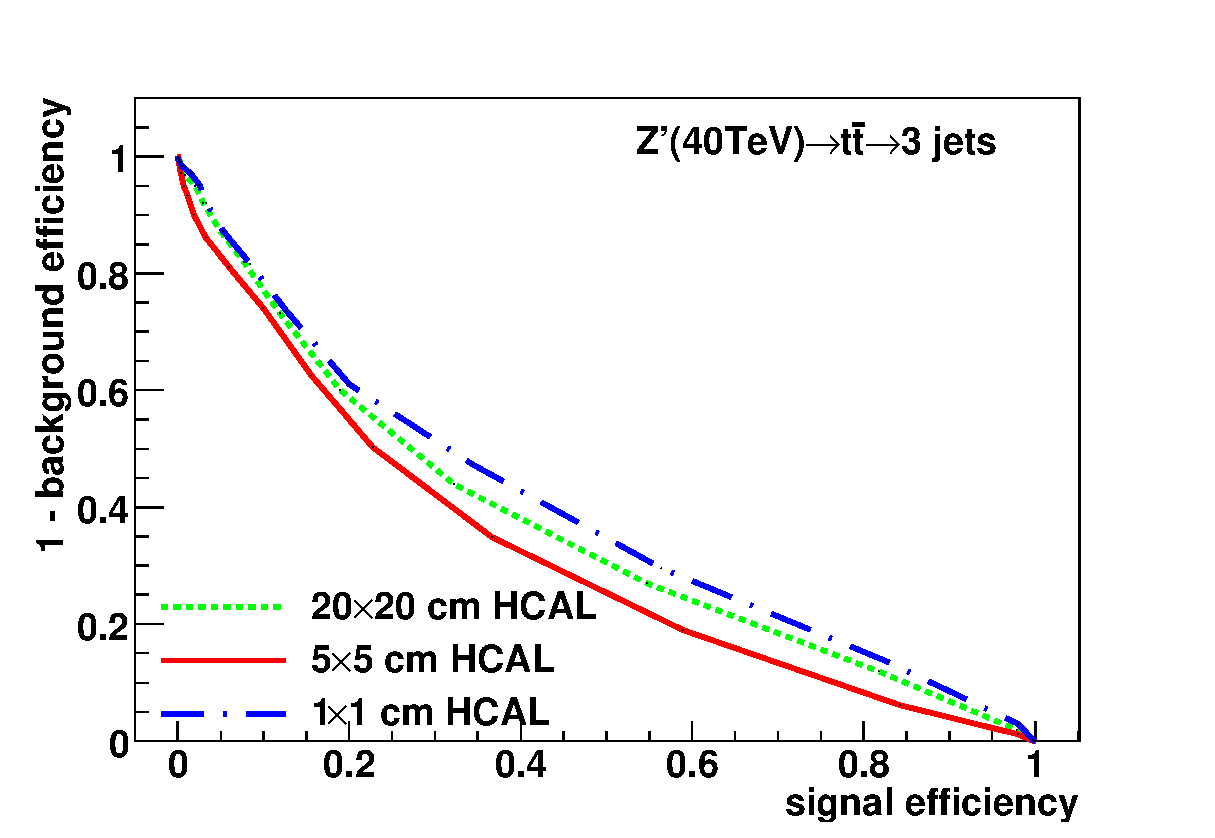
\includegraphics[width=0.43\textwidth]{figs/cluster_tau32_40_tev_eff.eps}
   }
\end{center}
\caption{Signal efficiency versus background rejection rate using $\tau_{32}$.The energies of collision at (a)5, (b)10, (c)20, (d)40TeV are shown here. In each picture of the energy, there are three ROC curves corresponding to different detector sizes.}
\label{fig:cluster_tau32}
\end{figure}

